%{\bf BME154L - Exam \#1}\hfill Name:\underline{\hspace*{3.0in}}



\section{How loud will this get?! [1 point]}
After a long day in the lab, you decide to go back to your dorm to setup
your new stereo system.  You bought one amplifier, but you weren't sure what
speakers to get, so you have 4 different models on hand.  The figure below
shows a simplified circuit schematic for your stereo amplifier and attached speaker.

\begin{figure}[h!]
\begin{minipage}[l]{0.8\linewidth}
\centering
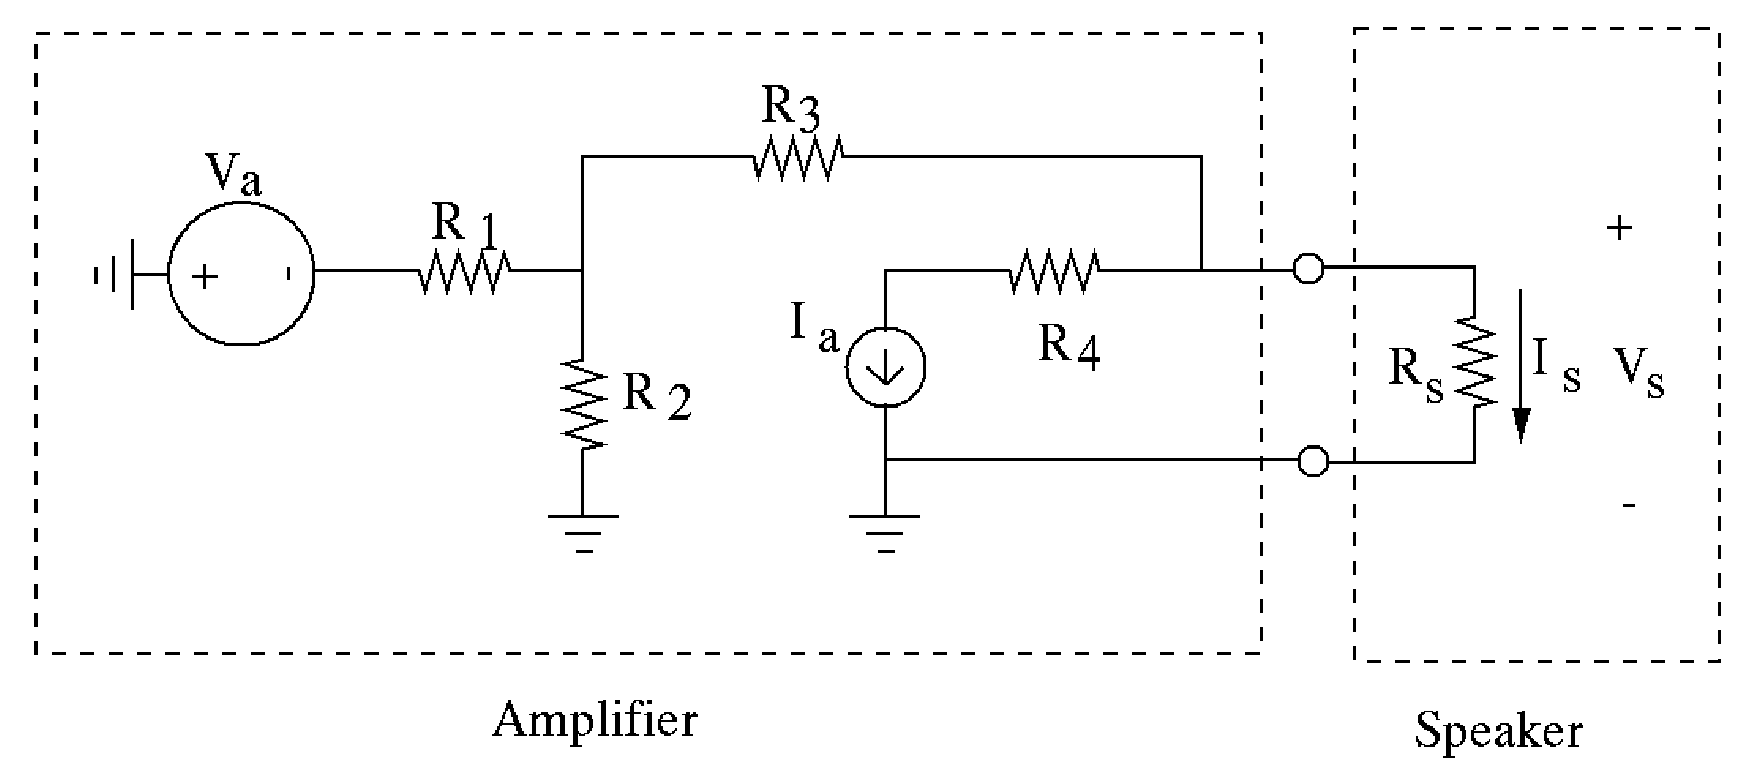
\includegraphics[width=5.0in]{p4/p4}
\caption{Amplifier/Speaker Stereo Circuit}
\label{fig:stereo}
\end{minipage}\hfill
\begin{minipage}[l]{0.2\linewidth}
\vspace*{-0.5in}
\begin{tabular}{|l|l|} \hline
Component & Value \\ \hline
$V_a$ & 10 V \\ \hline
$I_a$ & 5 A \\ \hline
$R_1$ & 6 $\Omega$ \\ \hline
$R_2$ & 6 $\Omega$ \\ \hline
$R_3$ & 5 $\Omega$ \\ \hline
$R_4$ & 3 $\Omega$ \\ \hline
\end{tabular}
\end{minipage}
\end{figure}

You pull out your handy ohmmeter in your dorm room an measure the resistance of
the 4 speakers that you bought, and you come up with the following values: $R_{S1}$ = 4 $\Omega$, $R_{S2}$ = 8 $\Omega$, $R_{S3}$ = 12 $\Omega$, $R_{S4}$ = 16 $\Omega$.

Given the amplifier circuit shown in Figure~\ref{fig:stereo}, what would
be the ideal speaker resistance ($R_{Si}$) to achieve maximum power delivery
from the amplifier?  (Hint: you don't need to solve the circuit for each value of $R_{Si}$)
\newpage
